% !TEX root =  ../report.tex
\section{Introduction}

This report aims to present the results of a heuristic usability evaluation for a prototype of a task management application, which is intended to aid users in organising their tasks, by providing the possibility to group them into lists that are placed on different boards. It was conducted together with partner groups and individuals, and it outlines the possible problems that could harm the overall experience of the user. The report will provide a guide-line of how the prototype was evaluated through fixed heuristics, it will describe the severity of the issues found and propose improvements based on the results. These heuristics outline a model for how a user-friendly app should behave, and comparing this app against them will assist in future design choices.

\graphicspath{{huereport/content/images/}}
\subsection{PROTOTYPE}
 The prototype that has undergone the evaluation is a partially functioning version of the whole application, showing an overview of the server selection scene, the board selection scene, the public board, the tag manager, and the adding card, board, and task scenes. In order for the reviewers to consider the application's current goals they also were showed mockups of intended design. Following are scenes from the prototype application all the reviewers got to use. The application has three intended use cases, out of which one is implemented in the prototype. These are:

\(\circ \) Accessing the server's public board, for example a manager posting announcements.

\(\circ \) Working on team board with colleagues.

\(\circ \) Using the private board for managing own tasks.
\newline
The app prototype starts with a server selection screen for users to connect to before proceeding to their work. They can then choose to join the public or private board, or go to the board selection scene to join or create a new team board. From there, users can enter the board overview to view all associated card lists.
\begin{figure}[H]
    \centering
    
\includegraphics[width=0.35\textwidth]{landing-page.png}
    \caption{Landing page}
    \label{fig:landing}
\end{figure}

\begin{figure}[H]
    \centering
    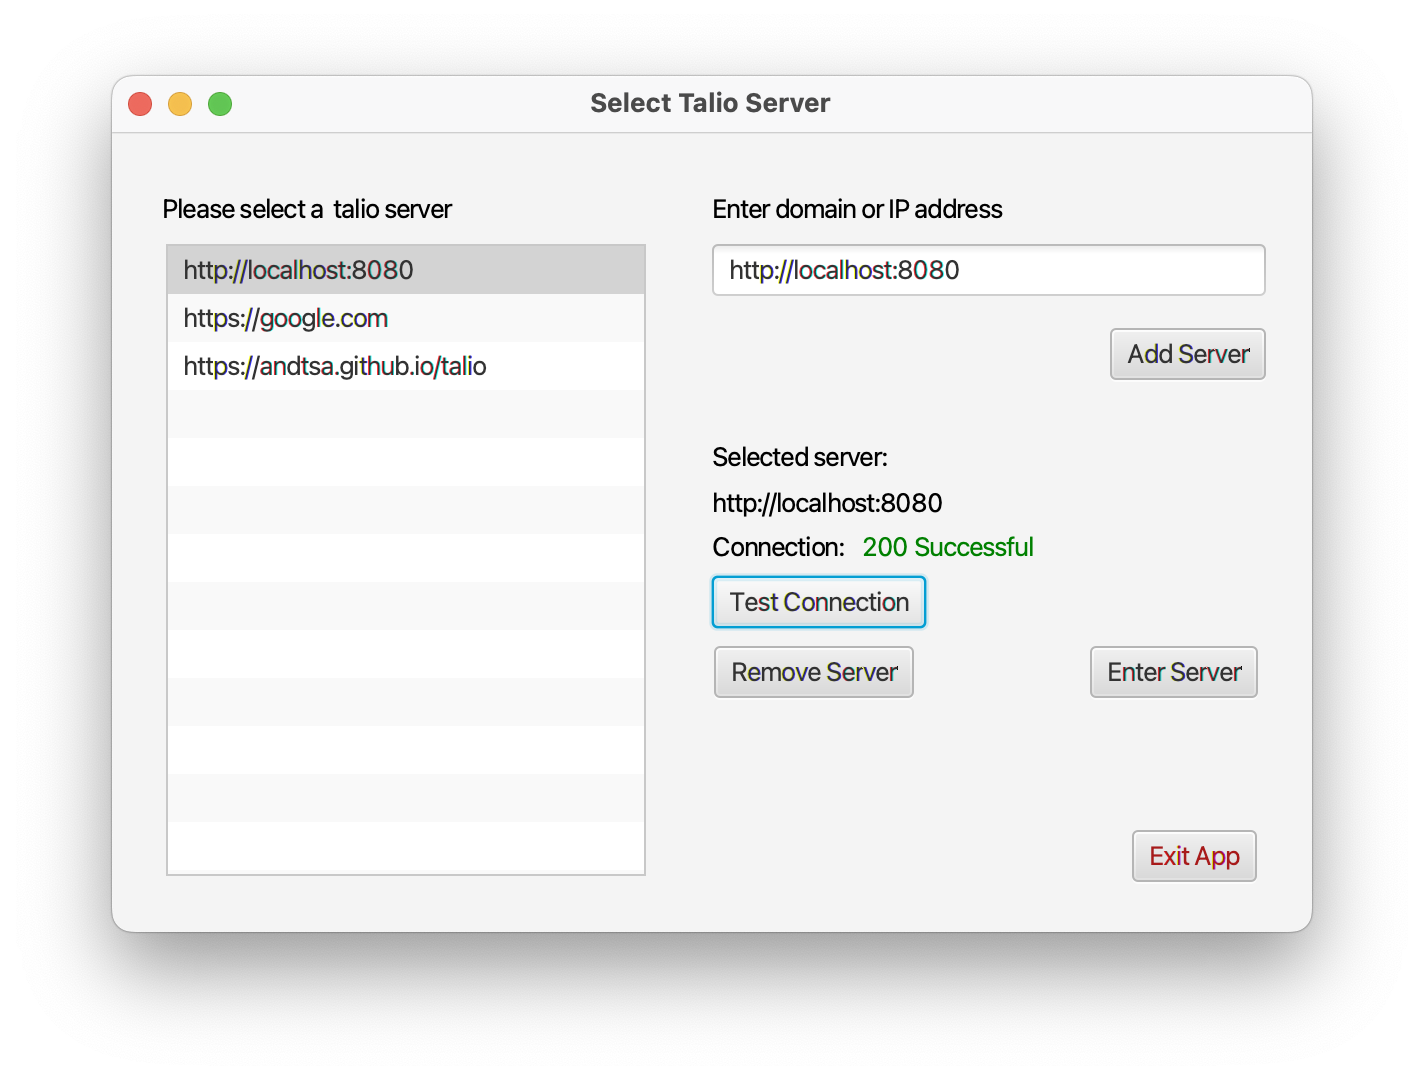
\includegraphics[width=0.35\textwidth]{test-connection-connected.png}
    \caption{Server Select}
    \label{fig:server}
\end{figure}

\begin{figure}[H]
    \centering
    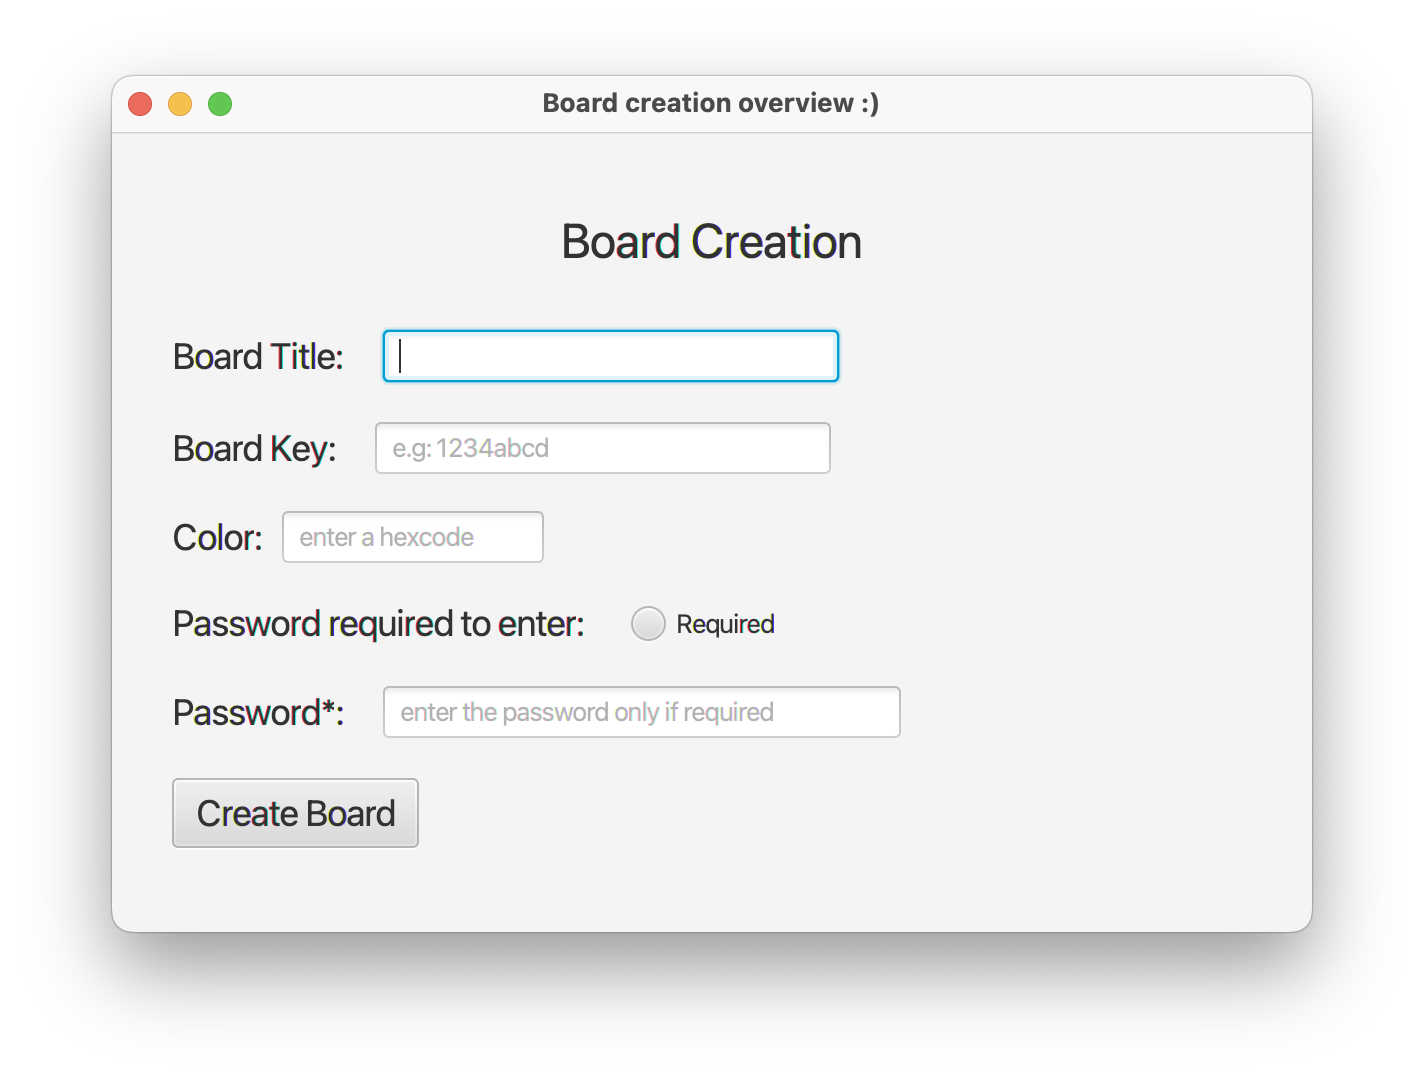
\includegraphics[width=0.35\textwidth]{board-creation.png}
    \caption{Board Creation}
    \label{fig:board-create}
\end{figure}

\begin{figure}[H]
    \centering
    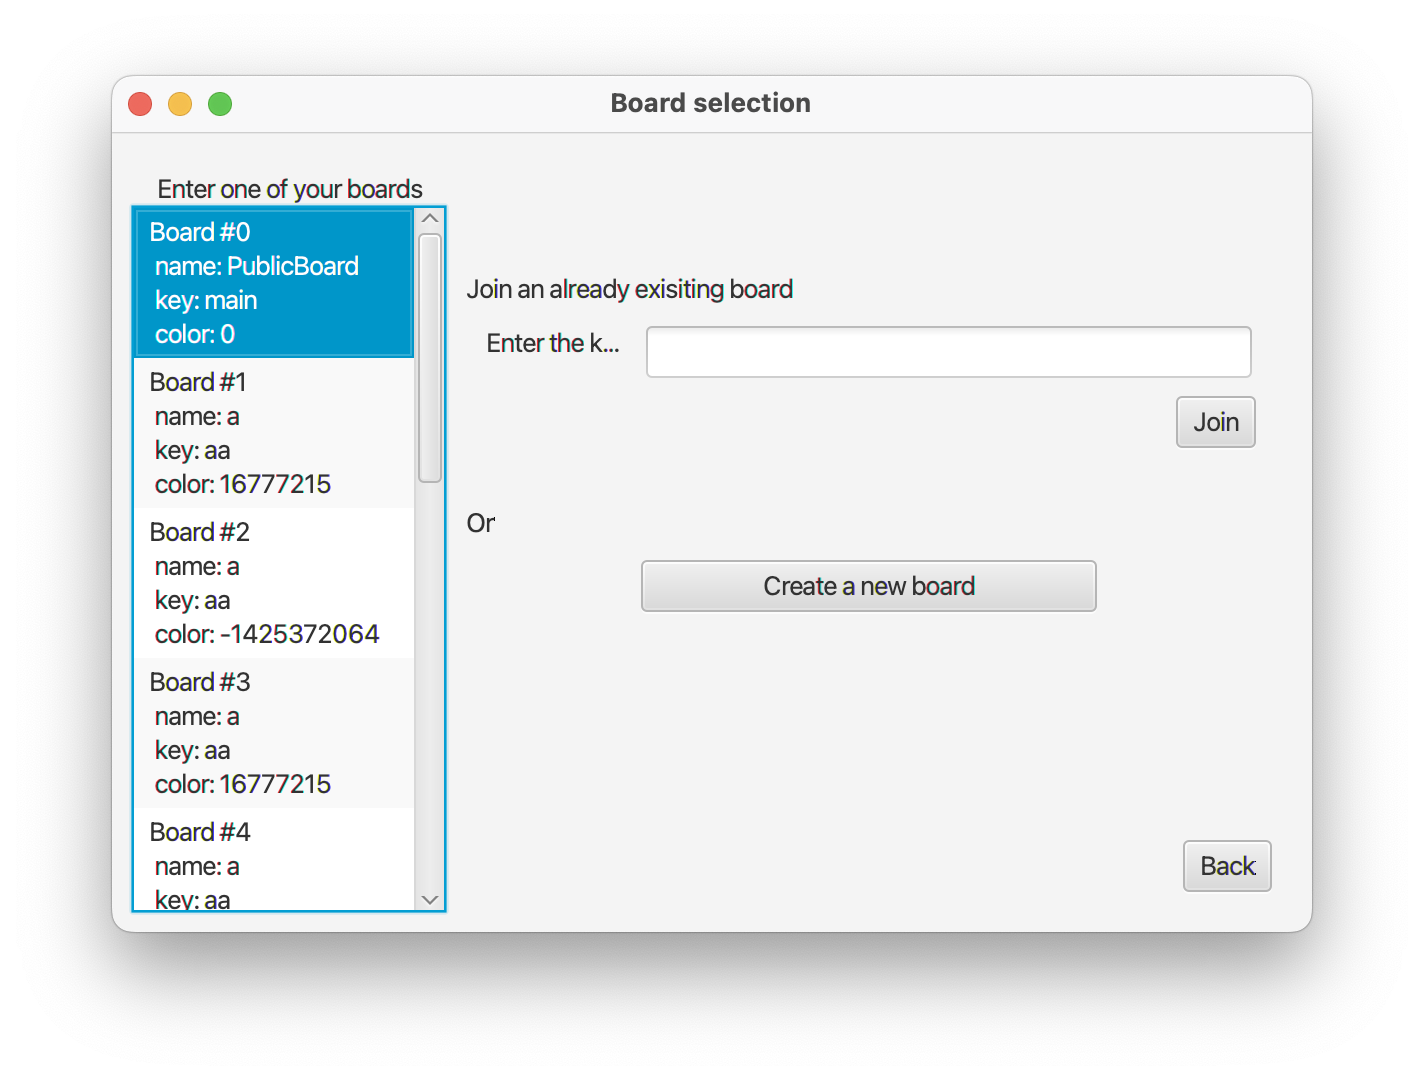
\includegraphics[width=0.35\textwidth]{board-selection.png}
    \caption{Board Select}
    \label{fig:board-select}
\end{figure}

\begin{figure}[H]
    \centering
    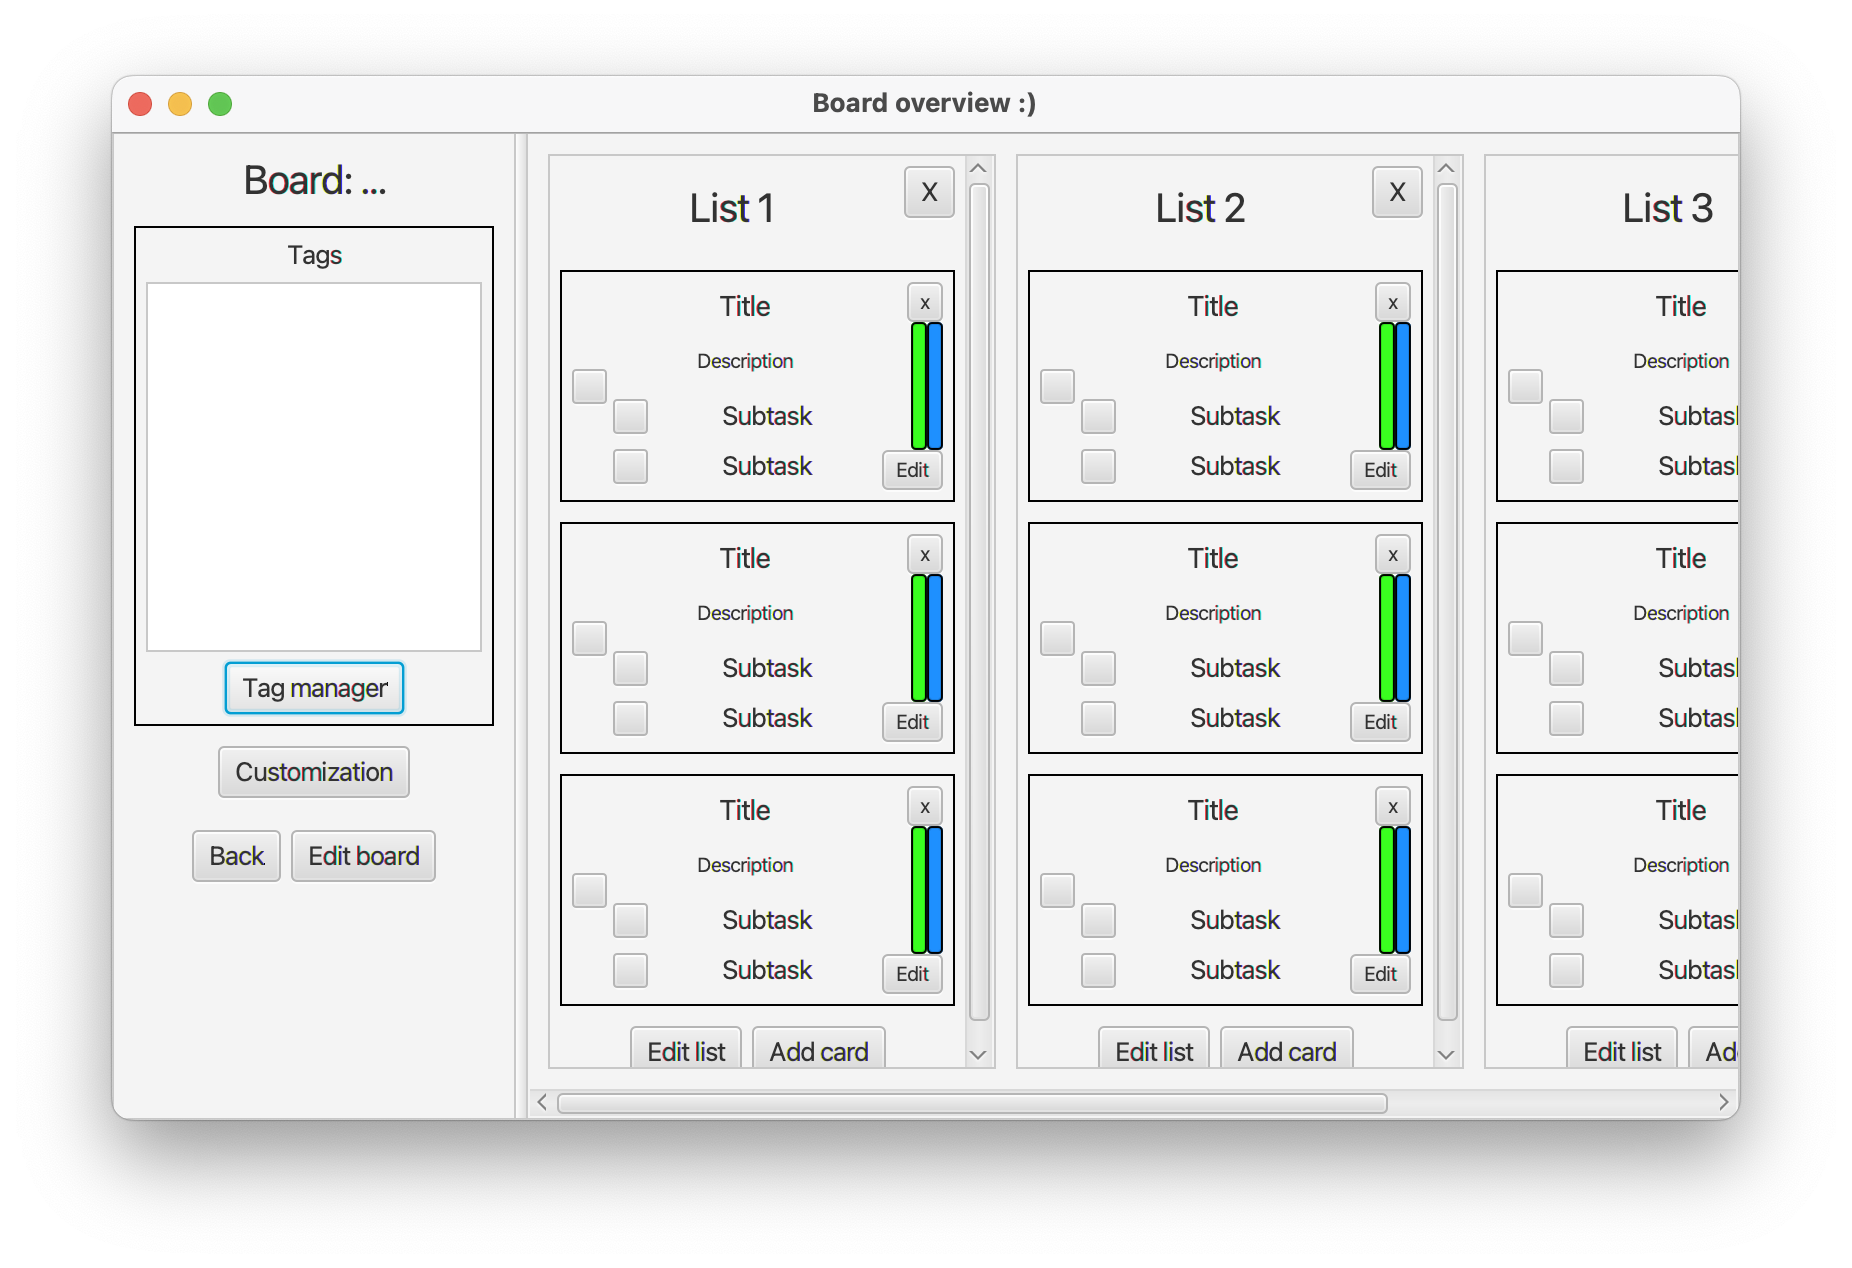
\includegraphics[width=0.35\textwidth]{board-overview.png}
    \caption{Board Overview}
    \label{fig:board-overview}
\end{figure}

\begin{figure}[H]
    \centering
    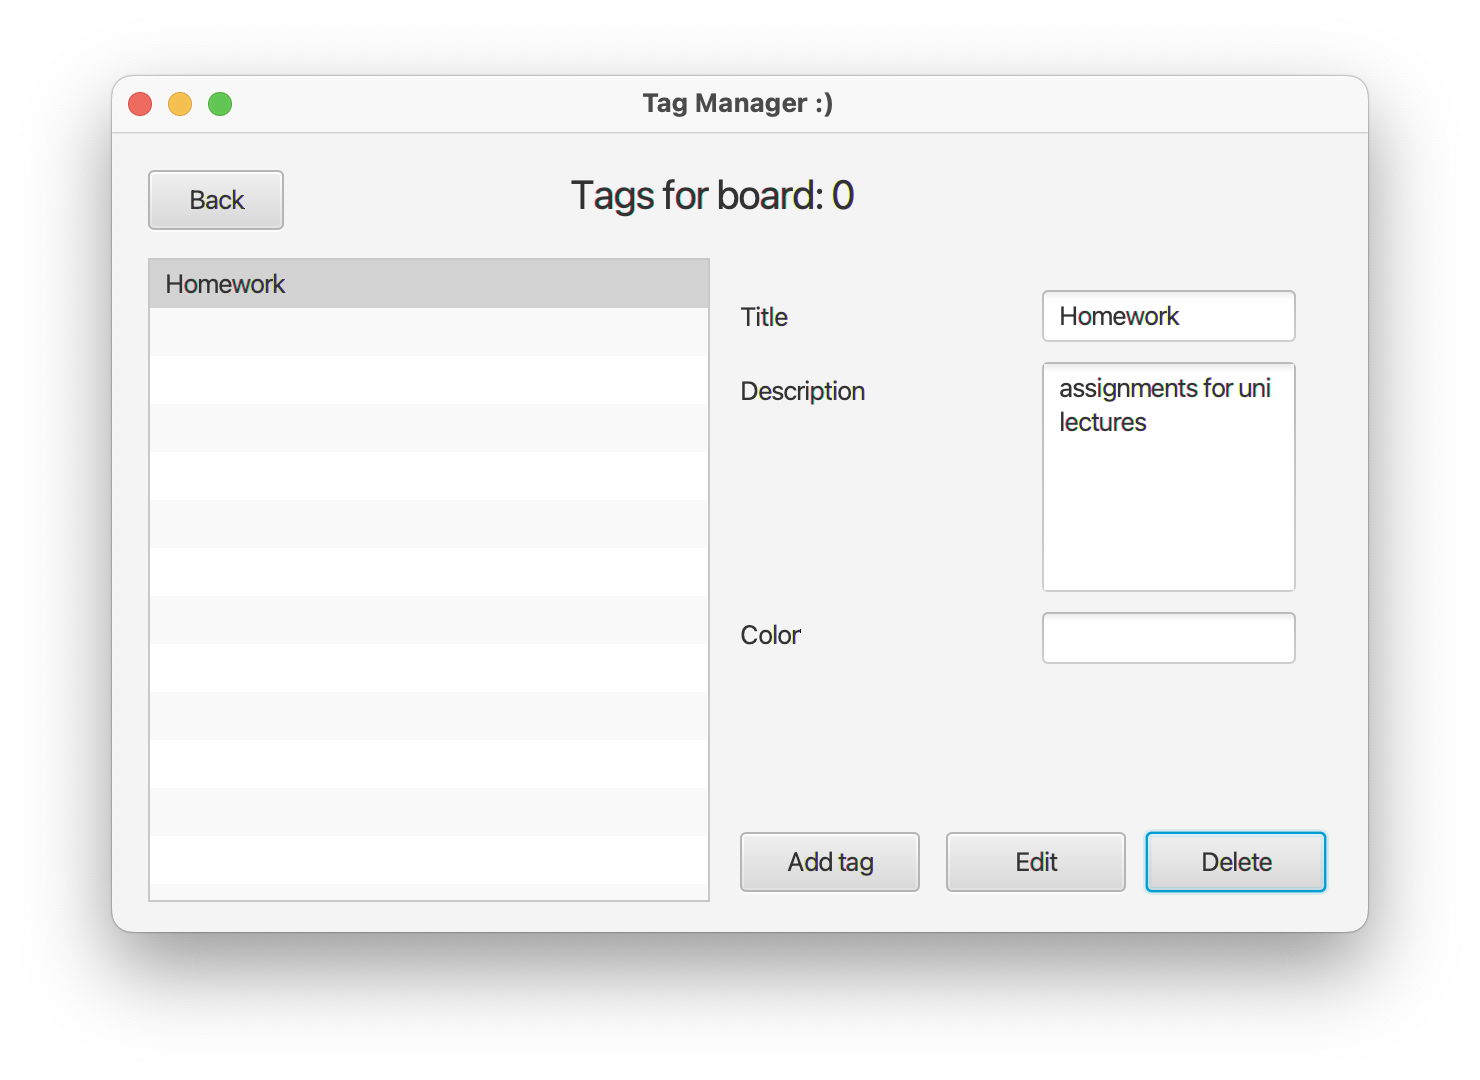
\includegraphics[width=0.35\textwidth]{tag-manager-one-tag.png}
    \caption{Tag Manager}
    \label{fig:tags}
\end{figure}

Taking into account that the application is in an early stage of development, the following mockups represent the guidelines the developers are following.

\begin{figure}[H]
    \centering
    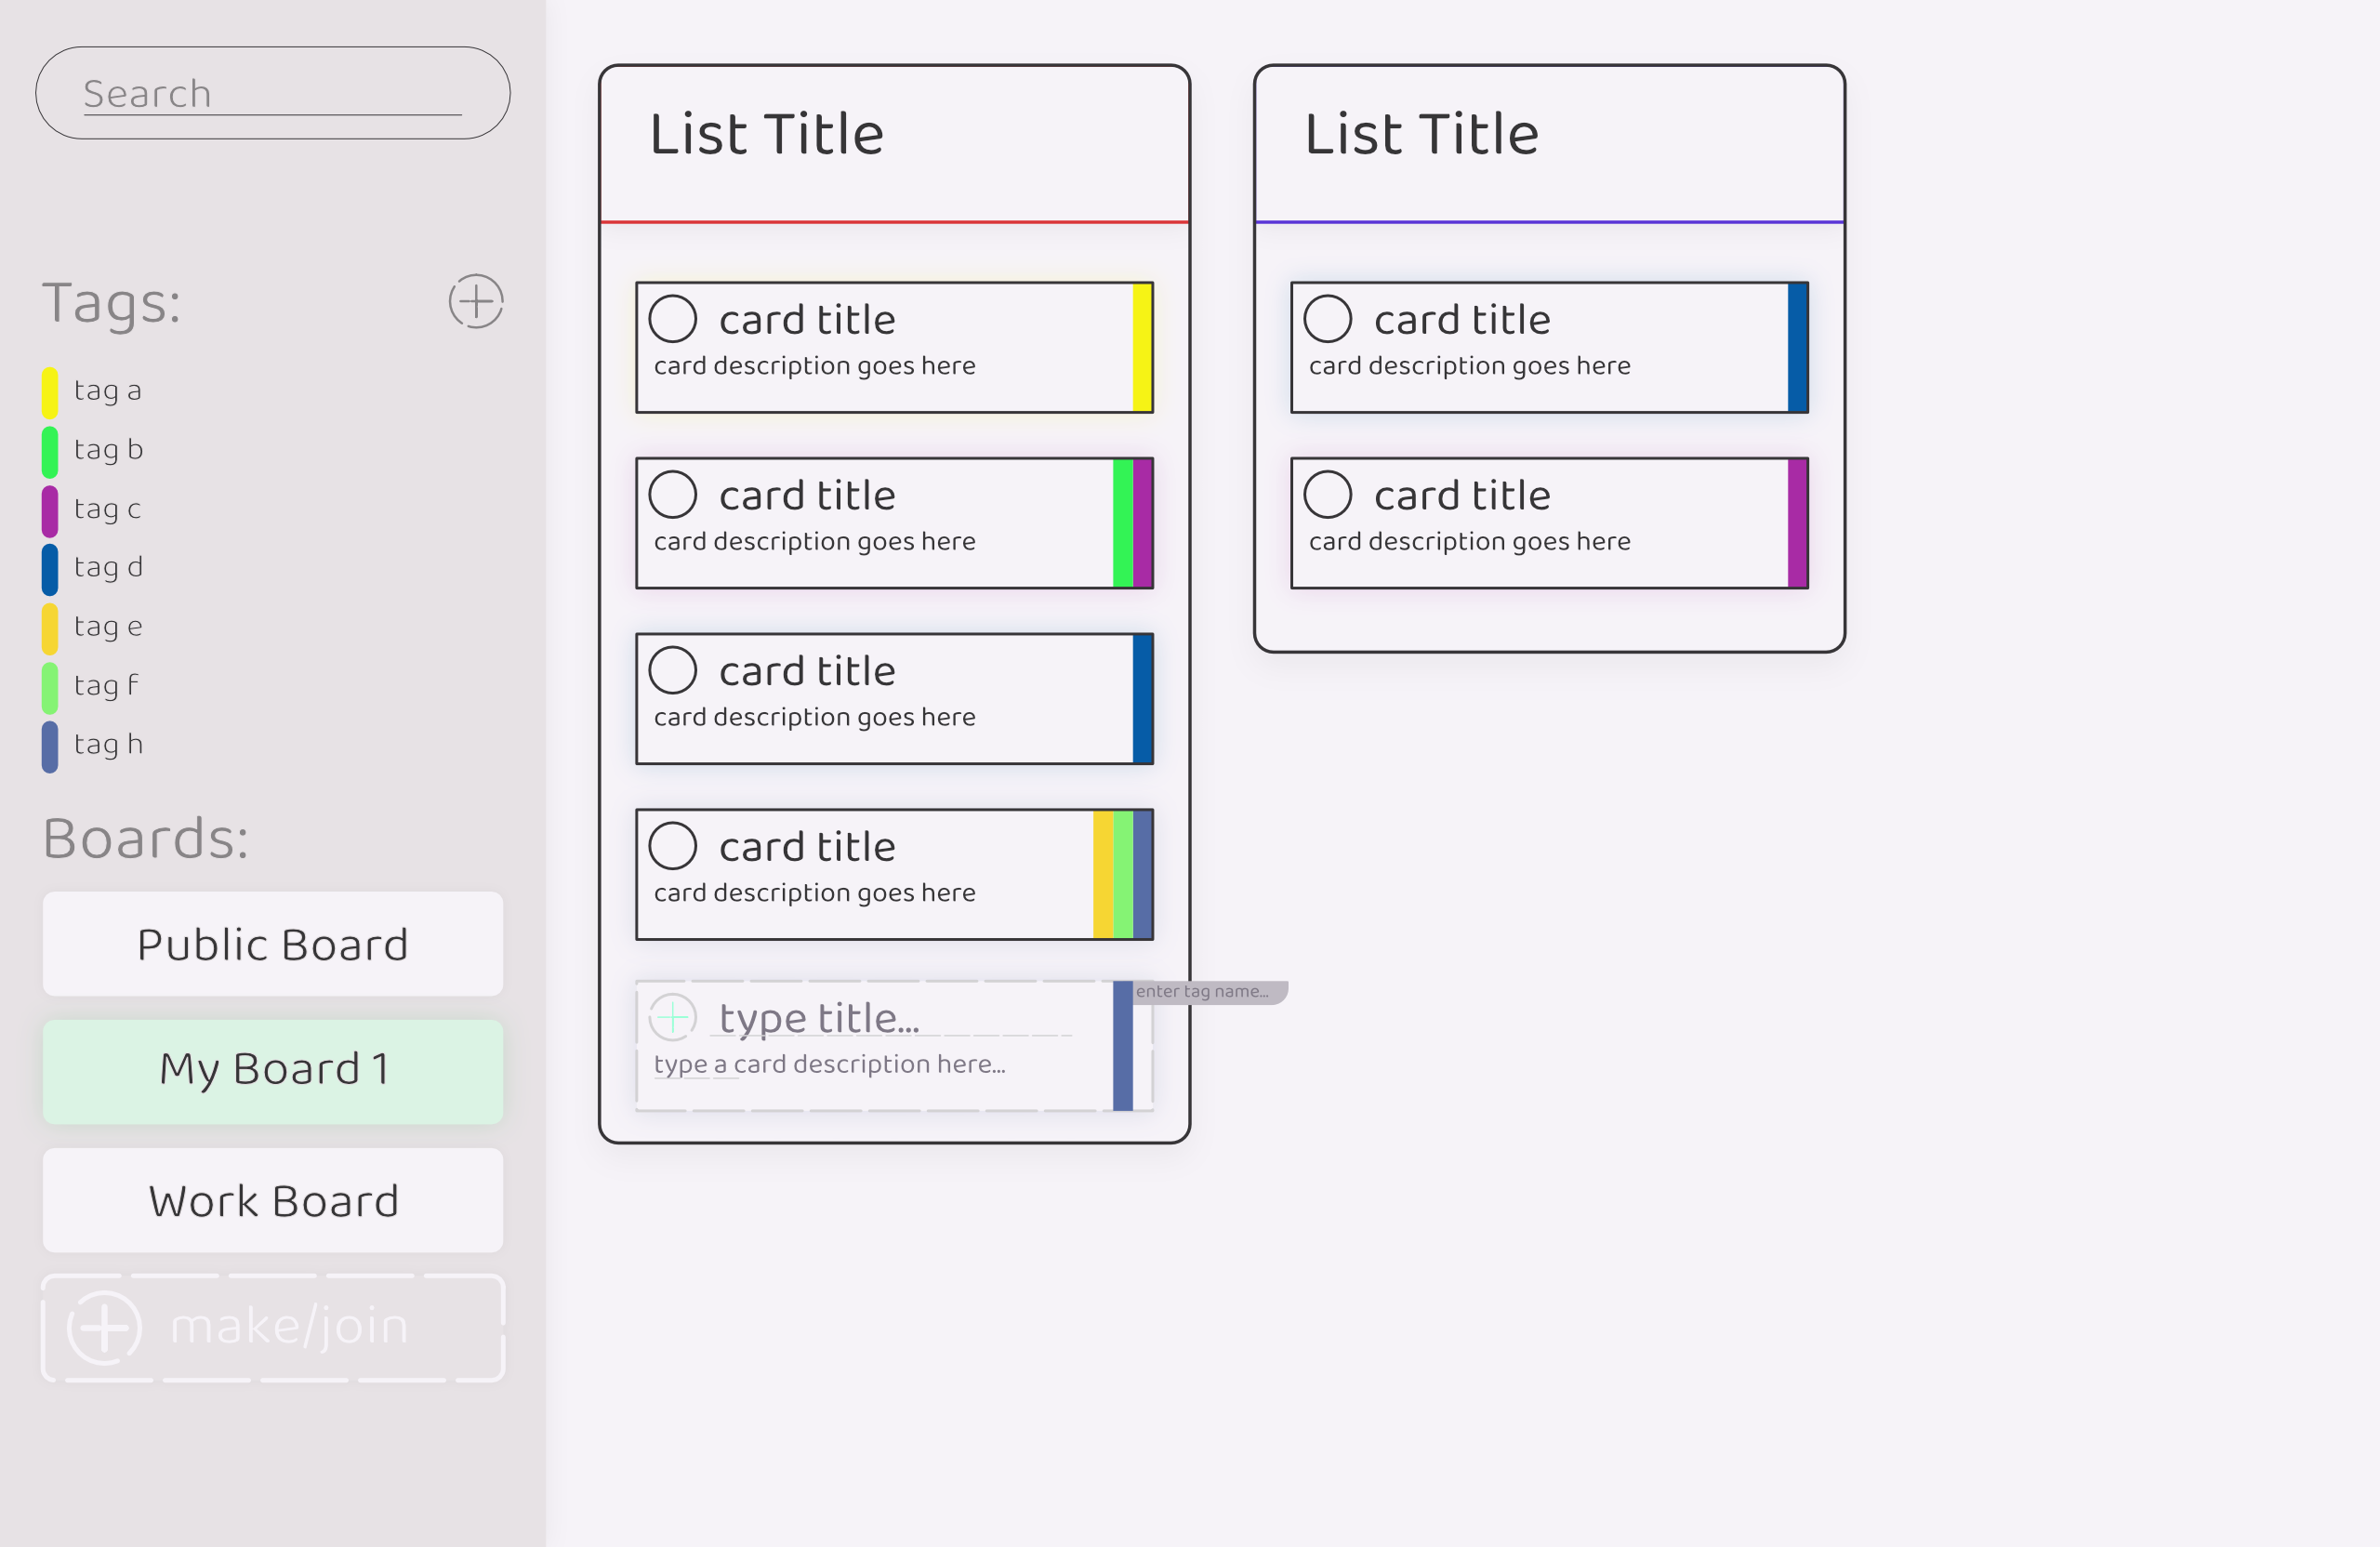
\includegraphics[width=0.4\textwidth]{mockup-1.png}
    \caption{Board Overview}
    \label{fig:mockup-overview}
\end{figure}

\begin{figure}[H]
    \centering
    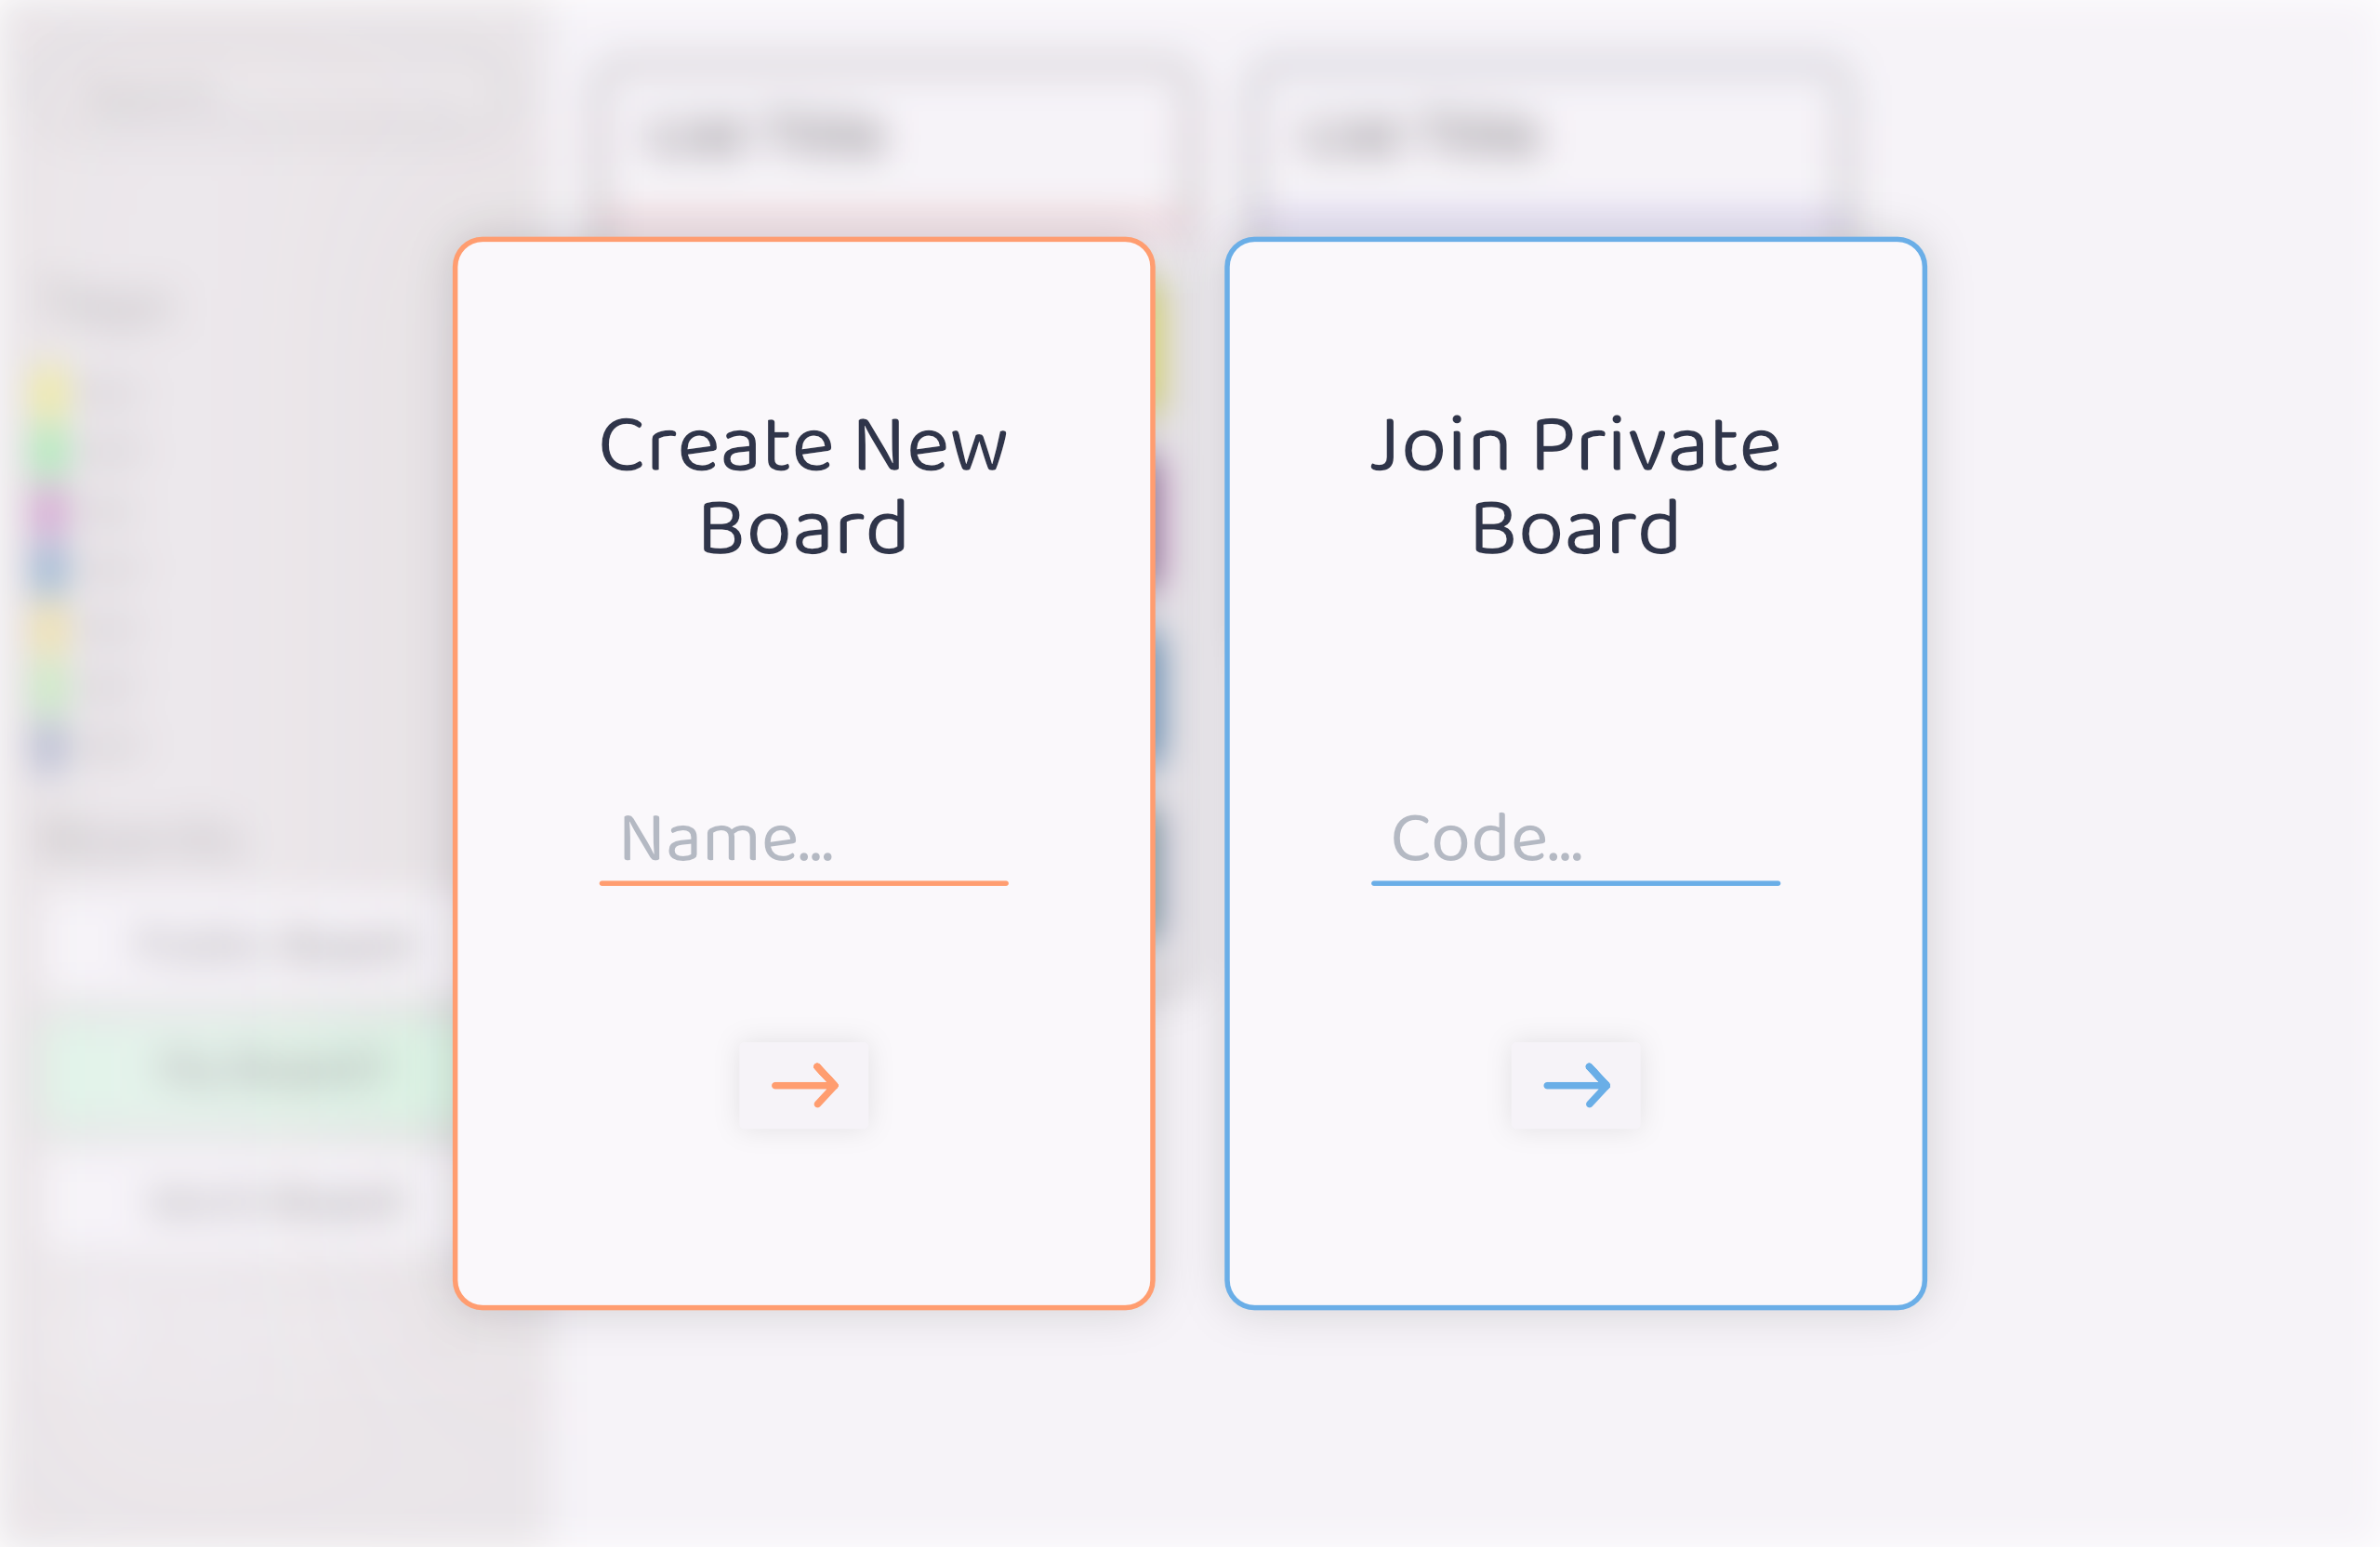
\includegraphics[width=0.4\textwidth]{mockup-2.png}
    \caption{Joining a new board}
    \label{fig:mockup-join}
\end{figure}